% \documentclass[draft]{beamer}
\documentclass[handout]{beamer}
% \documentclass{beamer}

\usepackage{amsmath,amssymb,amsthm}

% tikz includes
\usepackage{tikz}
\usepackage{animate}
\usetikzlibrary{decorations.pathreplacing}
\tikzstyle{every mynode}=[circle, draw, fill=black!50, inner sep=0pt, minimum width=4pt]

% beamer stuff
\usetheme{AnnArbor}
\usecolortheme{beaver}
\usefonttheme{professionalfonts}
\useinnertheme{rounded}
\useoutertheme{infolines}


\renewcommand{\emph}[1]{\textcolor{red}{#1}}
\newcommand{\mycolor}{red}

\title[Random Graphs]{Random Graphs and Zero-One Laws}
\subtitle{Strange Logic}
\author[J. Jung]{Jean Christoph Jung}
\institute[TdKI -- Uni Bremen]{Institut f\"ur Theorie der k\"unstlichen Intelligenz\\ Universit\"at Bremen}
\date{\today}
% \logo{\pgfimage[width=2cm,height=2cm]{hulogo}}
% \titlegraphic{\includegraphics[width=2cm,height=2cm]{hulogo}}
\subject{Random Graphs, Zero-One Laws, Logic}
\keywords{Random Graphs, Zero-One Laws, Logic}


\begin{document}

\titlepage

\begin{frame}{Outline}
\begin{enumerate}
\item Motivation
\item Random Graphs -- \emph{fixed} edge probability
\item Random Graphs -- \emph{variable} edge probability
% \item A Zero-One law for modal logic
\end{enumerate}
\end{frame}

\begin{frame}{Motivation}
Given first-order sentence $\varphi$ and an integer $n>0$. 

\begin{itemize}
\item What is the probability that $\varphi$ holds in a \emph{random} structure with domain size $n$?
\item What happens in the limit, \mbox{i.e.}, if $n\rightarrow\infty$?
\end{itemize}

\pause

Answer: in the limit, it is always 0 or 1!

\pause

Questions:
\begin{itemize}
\item What model of randomness do we use?
\item What happens in other logics, in particular modal logics?
\end{itemize}

\end{frame}

\begin{frame}{Model: constant edge probability}
\begin{itemize}
  \item restriction to one binary predicate E $\Rightarrow$ class of all (undirected) graphs 
  \item domain is $\{1,\ldots,n\}$
  \item $Pr( (u,v)\in E)=p$, $0<p<1$, independent from $(u',v')\neq(u,v)$
  \item yields probability distribution on the possible structures
  % \item first consider properties $A$ (instead of sentences)
  \item $\mu_n(A)$ is probability that property $A$ holds in a random graph of size $n$
  \item $A$ holds \emph{almost surely} if 
	$$\lim_{n\rightarrow\infty}\mu_n(A)=1$$
  \item notation: $G(n,p)$.
\end{itemize}
\end{frame}

\begin{frame}{Examples}
Assume $n=3$, $p=1/3$. We obtain the following distribution $G(n,p)$: 

\vspace{0.3cm}
\begin{columns}[t]
\column{1cm}
\column{3cm}
\begin{tikzpicture}[scale=1.4,
  mynode/.style={circle, draw, fill=black!50, inner sep=0pt, minimum width=4pt}]
  \draw (0,0) node[mynode] {};
  \draw (1,0) node[mynode] {};
  \draw (0.5,0.7) node[mynode] {};
\end{tikzpicture}

\vspace{0.3cm}
\hspace{0.4cm}
$\left(\frac{2}{3}\right)^3$
\column{3cm}
\begin{tikzpicture}[scale=1.4,
  mynode/.style={circle, draw, fill=black!50, inner sep=0pt, minimum width=4pt}]
  \draw (0,0) node[mynode] (a) {};
  \draw (1,0) node[mynode] (b) {};
  \draw (0.5,0.7) node[mynode] {};

  \draw (a) -- (b);
\end{tikzpicture}

\vspace{0.3cm}
$3\left(\frac{1}{3}\right)\left(\frac{2}{3}\right)^2$
\column{3cm}
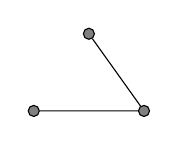
\begin{tikzpicture}[scale=1.4,
  mynode/.style={circle, draw, fill=black!50, inner sep=0pt, minimum width=4pt}]
  \draw (0,0) node[mynode] (a) {};
  \draw (1,0) node[mynode] (b) {};
  \draw (0.5,0.7) node[mynode] (c) {};
  \draw (a) -- (b) -- (c);
\end{tikzpicture}

\vspace{0.3cm}
$3\left(\frac{2}{3}\right)\left(\frac{1}{3}\right)^2$
\column{3cm}
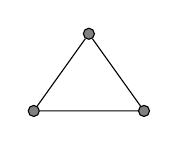
\begin{tikzpicture}[scale=1.4,
  mynode/.style={circle, draw, fill=black!50, inner sep=0pt, minimum width=4pt}]
  \draw (0,0) node[mynode] (a) {};
  \draw (1,0) node[mynode] (b) {};
  \draw (0.5,0.7) node[mynode] (c) {};
  \draw (a) -- (b) -- (c) -- (a);
\end{tikzpicture}

\vspace{0.3cm}
\hspace{0.4cm}
$\left(\frac{1}{3}\right)^3$
\end{columns}

\pause
\bigskip
\begin{center}
\begin{tabular}{lcc}
property $A$ & $\mu_3(A)$ & $\lim_{n\rightarrow\infty}\mu_n(A)$ \\
\hline
exists isolated vertex & 20/27 & 0 \\
\pause
exists path of length $2$ & 7/27 & 1\\
\pause
planarity & 1 & 0\\
\pause
triangle free & 26/27 & 0\\
\pause 
even number of vertices & 0 & -- 
\end{tabular}
\end{center}

\end{frame}

\begin{frame}{Theorem of Fagin - Glebskiy, Kogan, Liagonkii, Talanov}
For every first-order property $A$ we have
$$\lim_{n\rightarrow\infty}\mu_n(A)=0\mathrm{\ or\ } 1$$
\end{frame}


\begin{frame}{Proof -- The extension statement $A_{r,s}$}

\only<1-3>{
We define the property $A_{r,s}$ as follows:

\medskip
\hspace{0.5cm}for all distinct vertices $x_1,\ldots,x_r$, and $y_1,\ldots,y_s$
there exists a vertex \\\hspace{0.5cm}$z$ that is connected with all the $x_i$, but with none of the $y_i$.
}

\only<2->{
For arbitrary disjoint sets $X$, $Y$ with cardinality $r$, $s$:  

\begin{center}
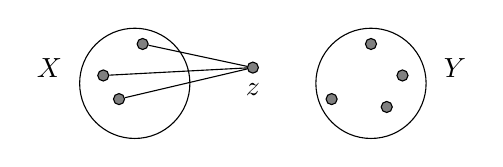
\begin{tikzpicture}
  [mynode/.style={circle, draw, fill=black!50, inner sep=0pt, minimum width=4pt}]
  \draw (2,0) circle (0.7cm);
  \coordinate [label=left:$X$] (X) at (1.2,0.2);
  \coordinate [label=right:$Y$] (Y) at (5.8,0.2);
  \draw (5,0) circle (0.7cm);
  \draw (2.1,0.5) node[mynode] (a) {};
  \draw (1.6,0.1) node[mynode] (b) {};
  \draw (1.8,-0.2) node[mynode] (c) {};
  \draw (5.0,0.5) node[mynode] {};
  \draw (5.4,0.1) node[mynode] {};
  \draw (4.5,-0.2) node[mynode] {};
  \draw (5.2,-0.3) node[mynode] {};

  \draw<3-> [fill=red] (3.5,0.2) node[mynode] (z) [label=below:$z$] {};
  \draw<3-> (z)--(a);
  \draw<3-> (z)--(b);
  \draw<3-> (z)--(c);
\end{tikzpicture}
\end{center}
}

\only<4->{
\medskip
Claim: $A_{r,s}$ holds almost surely for all $r,s\geq 0$.

\medskip
Proof: fix $x_1,\ldots,x_r$ and $y_1,\ldots,y_s$
\begin{itemize}
  \item<5-> for a fixed $z$: $Pr(x_i\sim z,y_i\not\sim z)=p^r(1-p)^s$
  \item<6-> $E=$"for no $z$ the extension holds". $P(E)=(1-p^r(1-p)^s)^{n-r-s}$
  \item<7-> set $\varepsilon=\min\{p,1-p\}^{r+s}$: $P(E)\leq(1-\varepsilon)^{n-r-s}$
  \item<8-> ${n\choose r}{n-r\choose s}$ choices for $x_1,\ldots,x_r$, and $y_1,\ldots,y_s$
  \item<9-> $P(\neg A_{r,s})\leq {n\choose r}{n-r\choose s}(1-\varepsilon)^{n-r-s}=O(n^{r+s})\cdot(1-\varepsilon)^{n-r-s}$
  \item<10-> in the limit: the right-hand-side goes to $0$
\end{itemize}
}
\end{frame}



\begin{frame}{Alice's Restaurant property}
  A graph that satisfies $A_{r,s}$ for all $r,s\geq 0$ fulfills \emph{Alice's Restaurant Property}.

  \begin{itemize}
    \item no finite graph has this property
    \item "counting argument" to show existence of countable graph
    \item back-and-forth argument to show uniqueness

    % \item call the unique graph $G_{rado}$
    % \item alternative existence proof: consider theory generated by $A_{r,s}$
  \end{itemize}

\pause
\bigskip
  SUPRISE: it is independent of $p$!!!

\pause
  We talk about THE random graph.
\end{frame}



\begin{frame}{Finishing the Proof using Logic}
  Consider $T=Th(\{A_{r,s}\mid r,s\geq 0\})$. By the previous slide we know: 
  \begin{itemize}
    \item no finite model
    \item unique countable model
  \end{itemize}
  $\Rightarrow$ $T$ is a complete theory, \mbox{i.e.}, for every FO-sentence $B$, either $B$ or $\neg B$ is provable. Suppose $B$ is provable
  \begin{itemize}[<+->]
    \item By Compactness, there is a finite proof, involving finitely many axioms $A^i$
    \item Any $G$ with $G\models B$ satisfies all $A^i$. 
    \item By complement: Any $G$ with $G\models \neg B$ satisfies $\bigvee_i\neg A^i$.
    \item $\mu_n(\neg B)\leq \sum_i\mu_n(\neg A^i)$. 
    \item For $n\rightarrow\infty$, the right-hand-side approaches $0$.
    \item Thus $B$ holds almost surely
  \end{itemize}
\end{frame}

\begin{frame}{Summing up}
  Again: $T=Th(\{A_{r,s}\mid r,s\geq 0\})$. 
  \begin{itemize}
    \item for every $B\in T$: $\lim_{n\rightarrow\infty} \mu_n(B)=1$
    \item for every $B\notin T$: $\lim_{n\rightarrow\infty} \mu_n(B)=0$
    \item Completeness of $T$ yields: for every sentence $A$ we have
  $$\lim_{n\rightarrow\infty}\mu_n(A)=0\mathrm{\ or\ } 1$$
    \pause
    \item Also by completeness, the above theory $T$ equals
      $$\{A\mid\lim_{n\rightarrow\infty}\mu_n(A)=1\}$$
    \pause
    \item Zero-One Law
  \end{itemize}

\end{frame}



\begin{frame}{Revisiting the Property "Triangle-Free"}
  Remember: $G(n,p)$ and $A$="$G$ contains no triangle"
  \pause
  \begin{itemize}
    \item probability that three vertices form a triangle: $p^3$
    \pause
    \item $X$ ... number of triangles in $G(n,p)$.
    \item the expected number of triangles: $E(X)={n \choose 3}\cdot p^3$
    \pause
    \item Observation: $E(X)\rightarrow\infty$ since $p$ is constant
    \item Take $p$ a function of $n$:  
	\begin{itemize}
	  \item for $1/n\in o(p)$: $E(X)$ goes to $\infty$ and $\mu_n(A)\rightarrow 0$
	  \pause
	  \item for $p\in o(1/n)$: $E(X)$ goes to $0$ and $\mu_n(A)\rightarrow 1$
          \pause
          \item What happens for $p(n)=c/n$? \pause\\some combinatorics gives: 
      $$\lim_{n\rightarrow\infty}\mu_n(A)=\lim_{n\rightarrow\infty}P(X=0)=e^{-c^3/6}$$
  	\end{itemize}
    \item $1/n$ is a \emph{threshold function} for $A$
  \end{itemize}
\end{frame}


\begin{frame}{Threshold functions}
  We write $f(n)\ll g(n)$ if $\lim_{n\rightarrow\infty} f(n)/g(n)=0$
  
\pause
\bigskip
  A function $f(n)$ is called \emph{threshold function} for a property $A$ if
  \begin{enumerate}
    \item for $p(n)\ll f(n)$, we have $\lim_{n\rightarrow\infty}\mu_n(A)=0$
    \item for $p(n)\gg f(n)$, we have $\lim_{n\rightarrow\infty}\mu_n(A)=1$
  \end{enumerate}

  \pause
  Example from previous slide $f(n)=c/n$, $A$ "triangle free": 

  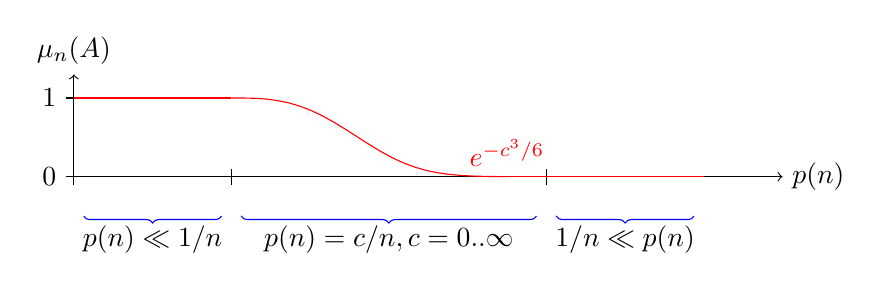
\begin{tikzpicture}[domain=0:3.5]
   \draw (-2,-0.5) node (a) {};
   \draw (0,-0.5) node (b) {};
   \draw (4,-0.5) node (c) {};
   \draw (6,-0.5) node (d) {};
   \draw[->] (-2.1,0) node[left] {0}-- (7,0) node[right] {$p(n)$};
   \draw[->] (-2,-0.1) -- (-2,1.3) node[above] {$\mu_n(A)$};
   \draw     (-2.1,1) node[left] {1} -- (-1.9,1);
   \draw     (0,-0.1) -- (0,0.1);
   \draw     (4,-0.1) -- (4,0.1);
   \draw[color=red] plot (\x,{exp(-0.16666*\x*\x*\x)}) node[above] {$e^{-c^3/6}$};
   \draw[color=red] (-2,1) -- (0,1);
   \draw[color=red] (3.5,0) -- (6,0);

   \draw[decorate,decoration={mirror, brace},blue] (a) -- node[color=black,below] {$p(n)\ll 1/n$} (b);
   \draw[decorate,decoration={mirror, brace},blue] (b) -- node[color=black,below] {$p(n)=c/n,c=0..\infty$} (c);
   \draw[decorate,decoration={mirror, brace},blue] (c) -- node[color=black,below] {$1/n\ll p(n)$} (d);
  \end{tikzpicture}
\end{frame}



\begin{frame}{Zero-One Laws \mbox{vs.} Threshold Functions}
  We say $p(n)$ satisfies the \emph{Zero-One Law}, if in $G(n,p(n))$, every
first order property $A$ holds either almost surely or almost never. 

\pause
\begin{itemize}
  \item $p(n)=const$ satisfies the Zero-One Law.
  \item $p(n)=c/n$ does not satisfy the Zero-One Law.
  \pause
  \item other functions??
		\pause
	\item $p(n)$ threshold for $A$ $\Rightarrow$ $p(n)$ does not satisfy the Zero-One Law 
		\pause
	\item not all first-order properties have a threshold function 
\end{itemize}

% \pause
% \emph{Note 1}: 
% 
% \pause
% \emph{Note 2}:
\end{frame}



\begin{frame}{Revisiting the "Triangle-Property" -- Again}
Remember the expected number $X$ of triangles in $G(n,p)$ was $E(X)={n\choose 3}p^3$.

\pause
\bigskip
\begin{itemize}
  \item Consider now an arbitrary graph $H$ with $v$ vertices and $e$ edges. 
  \item The potential number of copies of $H$ in $G(n,p)$ is $\sim c\cdot n^v$
  \item The expected number of copies is $\sim c\cdot n^v\cdot p^e$.
  \item If $p(n)\ll n^{-v/e}$, this goes to $0$ as $n$ grows
  \item If $p(n)\gg n^{-v/e}$, this goes to $\infty$ as $n$ grows\\
Does this mean $H$ appears almost surely? --\pause\ \emph{No!}
\end{itemize}
\begin{columns}
\column{3cm}
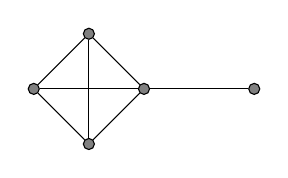
\begin{tikzpicture}[scale=1.4,
  mynode/.style={circle, draw, fill=black!50, inner sep=0pt, minimum width=4pt}]
  \draw (0,0) node[mynode] (a) {};
  \draw (1,0) node[mynode] (b) {};
  \draw (0.5,0.5) node[mynode] (c) {};
  \draw (0.5,-0.5) node[mynode] (d) {};
  \draw (2,0) node[mynode] (e) {};
  \draw (a) -- (c) -- (b) -- (d) -- (a);
  \draw (a) -- (b) -- (e);
  \draw (c) -- (d);
\end{tikzpicture}

\column{6cm}
$v/e=5/7$ but the $K_4$ is a subgraph with ratio $v'/e'=2/3<v/e$, so the $K_4$ appears "later".
\end{columns}
\end{frame}


\begin{frame}{The Evolution of the Random Graph $G(n,p(n))$}
	Idea: Let $p(n)$ increase -- what happens in $G(n,p(n))$?

	\begin{table}
		\centering
		\begin{tabular}{ll}
			$p(n)$ & threshold for (dis-)appearance of \\
			\hline
			$n^{-2}$ & isolated vertices \\
			$n^{-3/2}$ & paths of length $2$ \\
		\textcolor<2>{\mycolor}{$n^{-1-1/k}$} & \textcolor<2>{\mycolor}{trees with $k+1$ vertices} \\
			$n^{-1}$ & triangles, cycles of every finite length, planarity \\
			\textcolor<2>{\mycolor}{$n^{-v/e}$} & \textcolor<2>{\mycolor}{graphs with $e$ edges and $v$ vertices*} \\
			$\ln{n}/n$ & connectedness
		\end{tabular}
	\end{table}

	*: modulo previous slide

	$\Rightarrow$ for all of these $p$ there is no Zero-One Law!
\end{frame}



\begin{frame}{What happens in between $n^{-1-1/k}$ and $n^{-1-1/(k+1)}$?}
	Fix $k$ and assume
	$$n^{-1-\frac{1}{k}} \ll p(n) \ll n^{-1-\frac{1}{k+1}}$$

	One can show that in $G(n,p(n))$ almost surely: 
	\begin{itemize}
		\item There are no components with $k+2$ (or more) vertices.
		\item There are no cycles.
		\item For every $r$, every tree with  $1,\ldots,k+1$ vertices appears (at least) $r$ times.
	\end{itemize}

	\pause
	Consider the FO-theory $T$ of 1, 2, and 3. It has a unique countable model.

	$\Rightarrow T$ is complete 

	$\Rightarrow$ Zero-One Law for $G(n,p(n))$ 

	\bigskip
	\pause
	similar statements hold if $n^{-1-\varepsilon}\ll p(n) \ll n^{-1}$ for all $\varepsilon>0$
	or $n^{-1}\ll p(n) \ll n^{-1}\ln n$. 
\end{frame}

\begin{frame}{Between the rationals \dots}
	Already mentioned: $n^{-\alpha}$ is a threshold function for every rational $\alpha=a/b$,
	since at $n^{-a/b}$ graphs with $a$ vertices and $b$ edges appear almost surely.
	
	\pause
	\bigskip
	\textbf{Main Theorem} [Shelah, Spencer]: For every \emph{irrational} $\alpha$ with $0<\alpha<1$
	$p(n)=n^{-\alpha}$ satisfies a Zero-One Law, \mbox{i.e.}, in $G(n,n^{-\alpha})$ for every first-order $A$
	$$\lim_{n\rightarrow\infty}\mu_n(A)=0\mathrm{\ or\ } 1$$

	\pause
	\begin{itemize}
		\item theory $T_{\alpha}=\{A\mid \lim_{n\rightarrow\infty}\mu_n(A)=1\}$ is complete
		\item no unique countable model
		\item $T_{\alpha}$ is decidable (if $\alpha$ is)
		\item $T_{\alpha_1}\neq T_{\alpha_2}$ for $\alpha_1\neq\alpha_2$
	\end{itemize}
\end{frame}


\begin{frame}{Limiting probabilities}
	Assume that the Zero-One Law does not hold for $p(n)$.

	\pause
	\begin{itemize}
		\item Does the limit always exist? \\ \only<4->{\emph{[NonConvergence]}}
		\item If not, is it possible to seperate the cases when the limit is $0$ or $1$? \only<3->{\emph{[NonSeperability]}}
		\item If yes, what is the asymptotic probability of $A$ in $G(n,p(n))$? 
	\end{itemize}

	\only<5->{
	Two examples:
	\begin{itemize}
		\item $p(n)=c/n$: limit always exists, limit is a function of $c$ using $c$, $+$, $*$, and $exp(.)$
		\item $p(n)=n^{-1/3}$ limit does not always exist 
	\end{itemize}
	}
\end{frame}



\begin{frame}{}
	\begin{center}
		\LARGE{
		\emph{
		Thanks for your attention!
		}
		}
	\end{center}
\end{frame}


\end{document}
